\chapter{NUMERICAL SOLUTION}
\label{chap:numerical}
In this Chapter, the mathematical details involved in the numerical solution of the equations described in Chapters \ref{chap:kelp} and \ref{chap:light} are presented.
Two solution algorithms are used: finite difference and numerical asymptotics.
Both algorithms require a discrete spatial-angular grid, described in Section \ref{sec:grid}.
In the finite difference algorithm, the continuuum differential equation is approximated at every point in the grid.
This forms a large sparse system of linear equations which must be solved simultaneously with an iterative method.
The computational cost for this approach is high in terms of CPU usage, and especially in its memory requirement.

\section{Discrete Grid}
\label{sec:grid}

The following is a description of the spatial-angular grid used in the numerical implementation of this model.
It is assumed that all simulated quantities are constant over the interior of a grid cell.
Other legitimate choices of grids exist; this one was chosen for its relative simplicity.

The domain of the radiative transfer equation is embedded in five dimensions: three spatial ($x$, $y$, and $z$) and two angular (azimuthal $\theta$ and polar $\phi$).
The numbers of grid cells in each dimension are denoted $n_x$, $n_y$, $n_z$,
$n_\theta$, and $n_\phi$, with uniform spacings $dx$, $dy$, $dz$, $d\theta$, and
$d\phi$ between adjacent grid points.
Note that $n_\phi$ must be even in order to avoid perfectly horizontal rays, as discussed in Section \ref{sec:ray_notation} and Appendix \ref{chap:grid_details}.

The following indices are assigned to each dimension:
\begin{align*}
  x &\to i, \\
  y &\to j, \\
  z &\to k, \\
  \theta &\to l, \\
  \phi &\to m.
\end{align*}

It is convenient, however, to use a single index $p$ to refer to directions $\vec{\omega}$ rather than referring to $\theta$ and $\phi$ separately.
Then, the center of a generic grid cell will be denoted as
$(x_i, y_j, z_k, \vec{\omega}_p)$, and the boundaries between adjacent grid cells
will be referred to as \textit{edges}.
One-indexing is employed throughout this document (i.e., array elements are counted starting at 1, not 0).

\begin{figure}[H]
  \centering
  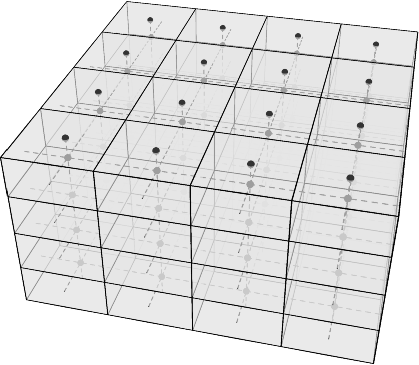
\includegraphics[width=8cm]{spatialgrid.pdf}
  \caption{Spatial grid. Discrete quantities are calculated at grid cell centers.}
  \label{fig:spatial_grid}
\end{figure}

Each spatial grid cell is the Cartesian product of $x$, $y$, and $z$ intervals of width $dx$, $dy$, and $dz$ respectively,
as shown in Figure \ref{fig:spatial_grid}.
The three-dimensional interval centered at $(x_i, y_j, z_k)$ is denoted $X_{ijk}$, and has volume $\abs{X_{ijk}}=dx\,dy\,dz$.
Also, note that no grid center is located on the plane $z=0$; the surface radiance boundary condition is treated separately.

\begin{figure}[H]
  \centering
  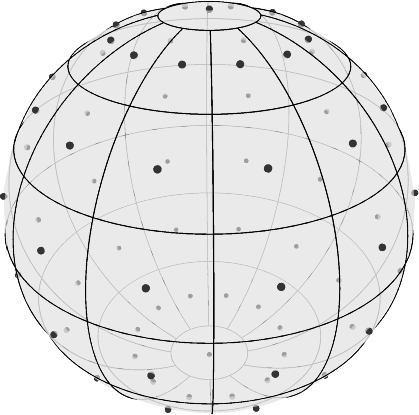
\includegraphics[width=8cm]{angulargrid.pdf}
  \caption{Angular grid at each point in space with poles treated separately.}
  \label{fig:angular_grid}
\end{figure}

As shown in Figure \ref{fig:angular_grid}, $\phi=0$ and $\phi=\pi$, called
the north ($+z$) and south ($-z$) poles respectively, are treated separately from other angular grid cells.
A generic interior angular grid cell centered at $\vec{\omega}_p$ is the Cartesian product of an azimuthal interval of width $d\theta$ and a polar interval of width $d\phi$.
However, the two pole cells are the Cartesian product of a polar interval of width $d\phi/2$ and the full azimuthal domain, $[0, 2\pi)$.

With this configuration, the total number of angles considered is $\nomega = n_\theta(n_\phi-2)+2$.
Then, cells are indexed by $p=1,\ldots,n_{\vec{\omega}}$ and are ordered such that
$p=1$ and $p=n_{\vec{\omega}}$ refer to the north and south poles respectively,
$p\leq\nomega/2$ refers to the northern hemisphere, and $p>\nomega/2$ refers to the southern hemisphere.
Further, the symbol $\Omega_p$ is used to refer to the two dimension angular interval centered at $\vec{\omega}_p$.
The solid angle subtended by $\Omega_p$ is denoted $\abs{\Omega_p}$.
The functions $\hat{p}(l,m)$, $\hat{l}(p)$, and $\hat{m}(p)$ are mappings between the two sets of angular indices.
Refer to Appendix \ref{chap:grid_details} for a more rigorous discussion of the discrete spatial-angular grid.

\section{Kelp Distribution}

\subsection{Super--Individuals}
\label{sec:si}

Rather than model each kelp frond, subsets of the population, called super-individuals, are modeled explicitly, and are considered to represent many identical individuals, as in \citep{scheffer_super-individuals_1994}.
Specifically, at each depth $k$, there are $S_k$ super-individuals, indexed by $q$.
Super-individual $q$ has a frond area $A_{kq}$ and represents $S_{kq}$ individual fronds.

From \eqref{eqn:length_from_area}, the frond length of the super-individual is $l_{kq} = \sqrt{2A_{kq}f_r}$.
Given the super-individual data, we calculate the mean $\mu$ and standard deviation $\sigma$ frond
lengths using the formulas
\begin{align}
  \mu_k &= \frac{\ds \sum_{q=1}^{S_k} l_{kq}}{\ds \sum_{q=1}^{S_k} S_{kq}},
  \label{eqn:si_mean} \\
  \sigma_k &= \frac{\ds \sum_{q=1}^{S_k} \left( l_{kq} - \mu_k \right)^2}{\ds \sum_{q=1}^{S_k} S_{kq}}.
  \label{eqn:si_std}
\end{align}
We then assume that frond lengths are normally distributed in each depth layer
with mean $\mu_k$ and standard deviation $\sigma_k$.

\subsection{Integration of Population Distributions}
The computational crux of calculating the kelp distribution is to evaluate \eqref{eqn:integrate_p2d} by integrating $P_{2D}(\theta_f, l)$ from \eqref{eqn:p2d} over the occupancy region $R_s(\theta, s)$, defined by \eqref{eqn:rs_th} and \eqref{eqn:rs_l}, for every point $(\theta,s)$ in the $xy$--domain.
To recap, the population distribution is
\begin{align*}
	P_{2D}(\theta_f,l) &= P_{\theta_f}(\theta_f) \cdot P_l(l), \\
  P_l(l) &= \frac{1}{\sqrt{2\pi\sigma_l^2}}\exp\left(\frac{-(l-\mu_l)^2}{2\sigma_l^2}\right), \\
	P_{\theta_f}(\theta_f) &= \frac{\exp\left(\eta v_w\cos(\theta_f-\theta_w)\right)}{2\pi I_0(\eta v_w)},
\end{align*}
and the occupancy region for $(\theta, s)$ is $R_s(\theta, s) = (\theta_f, l)$ such that
\begin{align*}
	\theta - \alpha &< \theta_f < \theta + \alpha, \\
	&l > l_{\min}(\theta,s).
\end{align*}

To compute the integral, we symbolically convert the two-dimensional integral to a one-dimensional integral in terms of the error function
\begin{equation}
  \erf(x) = \frac{2}{\sqrt{\pi}} \int_0^x e^{-t^2}\, dt,
\end{equation}
which is a built--in function in most programming languages, including Fortran.
So, we evaluate
\begin{align*}
	\tilde{P}_k(\theta, s) &= \int_{R_s(\theta,s)}P_{2D}(\theta_f,l)\, d\theta_f\, dl \\
  &= \int_{\theta-\alpha}^{\theta+\alpha}
  \int_{l_{min}(\theta,s)}^{\infty}
  P_{\theta_f}(\theta_f) \cdot P_l(l)
  \, dl\, d\theta_f, \\
  %
  &= \frac{1}{\sqrt{2\pi\sigma_l^2}}
  \int_{\theta-\alpha}^{\theta+\alpha}
  P_{\theta_f}(\theta_f)
  \int_{l_{min}(\theta,s)}^{\infty}
  \exp\left(\frac{-(l-\mu_l)^2}{2\sigma_l^2}\right)
  \, dl\, d\theta_f. \\
\end{align*}
The substitution $u=(l-\mu_l)/\sqrt{2\sigma_l^2};\; du=dl/\sqrt{2\sigma_l^2}$ produces
\begin{align*}
  \tilde{P}_k(\theta, s)
  &= \frac{1}{\sqrt{\pi}}
  \int_{\theta-\alpha}^{\theta+\alpha}
  P_{\theta_f}(\theta_f)
  \int_{\frac{l_{min}(\theta,s)-\mu_l}{\sqrt{2\sigma_l^2}}}^{\infty}
  e^{-u^{2}}\, du
  \, d\theta_f \\
  %
  &= \frac{1}{2}
  \int_{\theta-\alpha}^{\theta+\alpha}
  P_{\theta_f}(\theta_f)
  \left[1 - \erf\left(\frac{l_{min}(\theta,s)-\mu_l}{\sqrt{2\sigma_l^2}}\right)\right]
  d\theta_f
\end{align*}

Note that the above integrand can be explicitly evaluated at any value of $\theta_f$, and is not restricted to values on a discrete grid.
The integral is then evaluated numerically using a quadrature rule of any chosen degree.
At present, a Gauss-Legendre quadrature with degree 101 is applied.
If the quadrature degree is chosen too low (e.g. 5), the resulting distribution is marked by numerical artifacts including discontinuities.
Since the kelp calculation is orders of magnitude faster than the light field calculation, there is no issue with choosing a high quadrature degree.

\subsection{Gaussian Convolution}
In order to blur the kelp distribution as described in Section \ref{sec:gaussian_blur}, $P_k(x, y, z)$ is first calculated without blurring according to Equations \eqref{eqn:integrate_p2d} and \eqref{eqn:kelp_pk} at every point $(x_i, y_j)$ in each depth layer, which yields a matrix $P_{ij}^k = P_k(x_i, y_j, z)$.
Then, the discrete convolution of $P_{ij}^k$ with the Gaussian $K(x, y; \sigma_b)$ from Equation \eqref{eqn:gaussian_kernel} is numerically computed by the same process used to post--process pixelated image with a Gaussian blur.

Notice first that the integral from Equation \eqref{eqn:gaussian_blur} has infinite extent.
For numerical computation, a discrete grid with finite bounds must be chosen.
Specifically, an array of uniformly spaced quadrature points ($x'_{i'}, y'_{j'}$) is chosen for the integration variables $x'$ and $y'$ with spacings $dx$ and $dy$ to match the existing grid.
In order to capture the large majority of the Gaussian distribution, the number of quadrature points is each dimension is chosen to be
\begin{equation}
  n_K = 2r_K+1,
\end{equation}
where
\begin{equation}
  r_K = \ceil\left(\max\left(\frac{2\sigma_b}{dx}, \frac{2\sigma_b}{dy}\right)\right).
\end{equation}
Then, the quadrature points are
\begin{align*}
  x'_{i'} = (i'-r_K)dx, \quad i'=1,\ldots,n_k,
  y'_{j'} = (j'-r_K)dy, \quad j'=1,\ldots,n_k.
\end{align*}
The kernel is then evaluated at the quadrature points to form the matrix
\begin{equation*}
  K_{i'j'} = K\left(x'_{i'}, y'_{j'}; \sigma_b\right).
\end{equation*}
Note that the continuous $K(x, y; \sigma_b)$ is normalized only on the infinite plane;
the discrete $K_{ij}$ must therefore be re--normalized on the finite grid as
\begin{equation*}
  K_{i'j'} = \frac{K_{i'j'}}{\sum_{i',j'} K_{i'j'}}.
\end{equation*}
Then, letting
\begin{align*}
  \delta_x(i, i') = i - r_K + i'\mbox{ mod1 }n_x, \\
  \delta_y(j, j') = j - r_K + j'\mbox{ mod1 }n_y,
\end{align*}
the convolved kelp distribution $P_{ij}^{kb}$ is evaluated as
\begin{align*}
  P_{ij}^{kb} &= P_k^b(x_i, y_j, z; \sigma_b) \\
  &= \int_{-\infty}^{\infty} \int_{-\infty}^{\infty} K(x', y', z; \sigma_b) P_k(x_i-x', y_j-y', z)\, dx'\, dy' \\
  &= dx\, dy\, \sum_{i'=1}^{n_k} \sum_{j'=1}^{n_k} K\left(x'_{i'}, y'_{j'}, z; \sigma_b\right) P_k\left(x_i-x'_{i'}, y_j-y'_{j'}, z\right) \\
  &= dx\, dy\, \sum_{i'=1}^{n_k} \sum_{j'=1}^{n_k} K\left(x'_{i'}, y'_{j'}, z; \sigma_b\right) P_k\left(x_{\delta_x(i,i')}, y_{\delta_y(j,j')}, z\right) \\
  &= dx\, dy\, \sum_{i'=1}^{n_k} \sum_{j'=1}^{n_k} K\left(x'_{i'}, y'_{j'}, z; \sigma_b\right) P_{\delta_x(i,i'), \delta_y(j,j')}^k.
\end{align*}
That is, at each grid point $(x_i, y_j)$, a weighted sum of periodic--adjacent values is taken according to the Gaussian kernel in order to perform the blur.



\section{Quadrature Rules}
As a prerequisite to algorithm development, a few key integrals are calculated here.
Since it is assumed that all quantities are constant within a spatial-angular grid cell,
the midpoint rule is employed for both spatial and angular integration.
Presented here is a basic derivation of the formulas for integration in the spatial-angular grid.
Further details are found in Appendix \ref{chap:ray_tracing}.

\subsection{Spatial Quadrature}
Define the \textit{spatial characteristic function} as
\begin{equation*}
  \mathcal{X}^X_{ijk}(\vec{x}) = \begin{cases}
    1, & \vec{x} \in X_{ijk}, \\
    0, & \mbox{otherwise}.
  \end{cases}
\end{equation*}
The double integral of a function $f(\vec{x})$ over a depth layer $k$ is approximated as
\begin{align*}
  \int_\xmin^\xmax\int_\ymin^\ymax f(x, y, z_k)\, dy\, dx &\approx \int_\xmin^\xmax \int_\ymin^\ymax \sum_{i=1}^{n_x}\sum_{j=1}^{n_y} \mathcal{X}^X_{ijk}(x,y,z_k) f(x_i, y_j, z_k)\, dy\, dx \\
  &= \sum_{i=1}^{n_x}\sum_{j=1}^{n_y} f(x_i, y_j, z_k) \int_\xmin^\xmax \int_\ymin^\ymax \mathcal{X}^X_{ijk}(x,y,z_k) \, dy\, dx \\
  &= \sum_{i=1}^{n_x}\sum_{j=1}^{n_y} \abs{X_{ijk}} f(x_i, y_j, z_k) \\
  &= dx\, dy\, \sum_{i=1}^{n_x}\sum_{j=1}^{n_y} f(x_i, y_j, z_k).
\end{align*}
The path integral of $f(\vec{x})$ over a path $\vec{l}(s)$ from $s=0$ to $s=\tilde{s}$ is
\begin{align*}
  \int_0^{\tilde{s}} f(\vec{l}(s))\, ds &\approx \sum_{i=1}^{n_x}\sum_{j=1}^{n_y}\sum_{k=1}^{n_z} f(x_i, y_j, z_k)\, ds_{ijk},
\end{align*}
where $ds_{ijk}$ is the total path distance of $\vec{l}(s)$ through $X_{ijk}$.
Full details of the path integral algorithm for straight line paths are found in Appendix \ref{chap:ray_tracing}.

\subsection{Angular Quadrature}
Define the \textit{angular characteristic function} as
\begin{equation*}
  \mathcal{X}^\Omega_p(\vec{\omega}) = \begin{cases}
    1, & \vec{\omega} \in \Omega_p, \\
    0, & \mbox{otherwise}.
  \end{cases}
\end{equation*}
Then, the integral of a function $f(\vec{\omega})$ over all angles is approximated as
\begin{align*}
  \int_{4\pi} f(\vec{\omega})\, d\vec{\omega} &\approx \int_{4\pi} \sum_{p=1}^\nomega f(\vec{\omega}_p) \mathcal{X}^\Omega_p(\vec{\omega})\, d\vec{\omega} \\
  &= \sum_{p=1}^\nomega f(\vec{\omega}_p) \int_{4\pi} \mathcal{X}^\Omega_p(\vec{\omega})\, d\vec{\omega} \\
  &= \sum_{p=1}^\nomega f(\vec{\omega}_p) \int_{\Omega_p} d\vec{\omega} \\
  &= \sum_{p=1}^\nomega f(\vec{\omega}_p) \abs{\Omega_p}.
\end{align*}
Similarly, the amount of light scattered between angular grid cells is found by integrating $\beta$ over specific regions.
Consider two angular grid cells, $\Omega_p$ and $\Omega_{p'}$.
Since $\beta(\vec{\omega}\cdot\vec{\omega}')$ is the probability density of scattering between $\vec{\omega}$ and $\vec{\omega}'$, the average probability density of scattering from $\vec{\omega} \in \Omega_p$ to $\vec{\omega}' \in \Omega_{p'}$ (or vice versa) is
\begin{equation*}
  \beta_{pp'} = \frac{1}{\abs{\Omega_p}\abs{\Omega_{p'}}} \int_{\Omega_p}\int_{\Omega_{p'}}\beta(\vec{\omega}\cdot\vec{\omega}')\, d\vec{\omega'}\, d\vec{\omega} \approx \beta(\vec{\omega}\cdot\vec{\omega}'),
\end{equation*}
assuming that $\beta$ is approximately constant over $\Omega_p$ and $\Omega_{p'}$.
Denote the radiance at $(x_i, y_j, z_k, \vec{\omega}_p)$ by $L_{ijkp}$.
Then, the total radiance scattered into $\Omega_p$ from $\Omega_{p'}$ is
\begin{align*}
  \int_{\Omega_p}\int_{\Omega_{p'}}\beta(\vec{\omega} \cdot \vec{\omega}')L(\vec{x},\vec{\omega}')\, d\vec{\omega}'\, d\vec{\omega}
  &\approx L_{ijkp'} \int_{\Omega_p}\int_{\Omega_{p'}} \beta(\vec{\omega} \cdot \vec{\omega}')\, d\vec{\omega}'\, d\vec{\omega} \\
  &= \beta_{pp'}\abs{\Omega_p}\abs{\Omega_{p'}}L_{ijkp'}.
\end{align*}
Hence, the average radiance scattered from $\Omega_{p'}$ into some $\vec{\omega} \in \Omega_p$ is $\beta_{pp'}\abs{\Omega'}L_{ijkp'}$.
Therefore, the radiance gain due to scattering into $\vec{\omega}_p$ from all other angles is
\begin{equation}
  \int_{4\pi}\beta(\vec{\omega_p}\cdot\vec{\omega_{p'}})L(\vec{x}, \vec{\omega}')\, d\vec{\omega} \approx \sum_{p=1}^\nomega \beta_{pp'}\abs{\Omega'}L_{ijkp}.
  \label{eqn:scatter_integral}
\end{equation}

\section{Numerical Asymptotics}
\label{sec:num_asymptotics}
The asymptotic approximations \eqref{eqn:asymptotics_soln_0} and \eqref{eqn:asymptotics_soln_n} to the radiative transfer equation \eqref{eqn:rte} are evaluated numerically as follows.
Given a position $\vec{x}$ and direction $\vec{\omega}$, a path through the discrete grid can be constructed using the ray tracing algorithm described in Appendix \ref{chap:ray_tracing}.
Let $\nu=1,\ldots,N\nobreak-\nobreak1$ index the spatial grid cells traversed (wholly or partially) by the ray, and define the \textit{path--length characteristic function}
\begin{equation*}
  \mathcal{X}^l_\nu(s) = \begin{cases}
    1, & s_\nu \leq s < s_{\nu+1}, \\
    0, & \mbox{otherwise},
    \end{cases}
\end{equation*}
where $s \in [s_\nu, s_{\nu+1}]$ parameterizes the path segment traversing cell $\nu$ and $ds_\nu = s_{\nu+1} - s_\nu.$ is the length of the segment.
Then, the piecewise constant representations of the path absorption coefficient $\tilde{a}(s)$ and the effective source $\tilde{g}_n(s)$ from Section \ref{sec:asymptotic_sol} are
\begin{align*}
  \tilde{g}_n(s) &= \sum_{\nu=1}^{N-1}\tilde{g}_{n\nu}\mathcal{X}^l_\nu(s), \\
  \tilde{a}(s) &= \sum_{\nu=1}^{N-1}\tilde{a}_{\nu}\mathcal{X}^l_\nu(s).
\end{align*}

Given $s$, the index of the next edge crossing is
\begin{equation*}
  \hat{\nu}(s) = \min\left\{ \nu \in \{1,\ldots,N\} : s_\nu>s \right\},
\end{equation*}
and the path length between $s$ and the next edge crossing is
\begin{equation*}
  \tilde{d}(s) = s_{\hat{\nu}(s)}-s.
\end{equation*}
Then, evaluating \eqref{eqn:asymptotics_soln_n} at $s=\tilde{s}$ is calculated as
\begin{align*}
  u_n(\tilde{s}) &= \int_0^{\tilde{s}}\tilde{g}_n(s')\exp\left( -\int_{s'}^{\tilde{s}}\tilde{a}(s'')\,ds'' \right)\, ds' \\
  &= \int_0^{\tilde{s}} \sum_{\nu=1}^{N-1}\tilde{g}_{n\nu}\mathcal{X}^l_\nu(s') \exp\left( -\int_{s'}^{\tilde{s}}\sum_{j=1}^{N-1}\tilde{a}_{j}\mathcal{X}^l_j(s'')\,ds'' \right)\, ds' \\
  &= \sum_{\nu=1}^{N-1}\tilde{g}_{n\nu}\int_0^{\tilde{s}} \mathcal{X}^l_\nu(s') \exp\left( -\sum_{j=1}^{N-1}\tilde{a}_{j}\int_{s'}^{\tilde{s}}\mathcal{X}^l_j(s'')\,ds'' \right)\, ds' \\
  &= \sum_{\nu=1}^{N-1}\tilde{g}_{n\nu}\int_{s_\nu}^{s_{\nu+1}}  \exp\left(-\tilde{a}_{\hat{\nu}(s')-1}\tilde{d}(s') -\sum_{j=\hat{\nu}(s')}^{N-1}\tilde{a}_{j}ds_j\right)\, ds' \\
  &= \sum_{\nu=1}^{N-1}\tilde{g}_{n\nu}\int_{s_\nu}^{s_{\nu+1}}  \exp\left(-\tilde{a}_{\nu}(s_{\nu+1}-s') -\sum_{j=\nu+1}^{N-1}\tilde{a}_{j}ds_j\right)\, ds'.
\end{align*}
This integral is made straightforward by setting
\begin{equation*}
  b_\nu = -\tilde{a}_{\nu}s_{\nu+1} - \sum_{j=\nu+1}^{N-1}\tilde{a}_{j}ds_j,
\end{equation*}
which yields
\begin{align*}
  u_n(\tilde{s}) &= \sum_{\nu=1}^{N-1}\tilde{g}_{n\nu}\int_{s_\nu}^{s_{\nu+1}}  \exp\left(\tilde{a}_{\nu}s' + b_\nu\right)\, ds' \\
                 &= \sum_{\nu=1}^{N-1}\tilde{g}_{n\nu}e^{b_\nu}\int_{s_\nu}^{s_{\nu+1}}  \exp\left(\tilde{a}_{\nu}s'\right) ds'.
\end{align*}
Define the intermediate variable
\begin{align*}
  d_\nu &= \int_{s_\nu}^{s_{\nu+1}}  \exp\left(\tilde{a}_{\nu}s'\right)\, ds' \\
    &= \begin{cases}
    ds_\nu, & \tilde{a} = 0 \\
      \left( \exp(\tilde{a}_\nu s_{\nu+1}) - \exp(\tilde{a}_\nu s_\nu) \right)/\tilde{a}_\nu, & \mbox{otherwise},
    \end{cases}
\end{align*}
which permits the simple formula
\begin{equation}
  u_n(\tilde{s}) = \sum_{\nu=1}^{N-1} \tilde{g}_{n\nu}d_\nu e^{b_\nu}.
  \label{eqn:discrete_ray_integral}
\end{equation}

When $n=0$, the boundary condition must be included for downwelling light,
and the effective source $\tilde{g}_{n\nu}$ is reduced to the explicit source $\tilde{\sigma}_{0\nu}$
for lack of a scattering term.
Thus, the numerical solution to \eqref{eqn:asymptotics_soln_0} is given by
\begin{align}
  u_0(\tilde{s}) &= f(\vec{\omega})H(\vec{\omega}\cdot\hat{z}) \exp\left( -\sum_{j=1}^{N-1}\tilde{a}_jds_j\right)
  + \sum_{\nu=1}^{N-1} \tilde{\sigma}_{0\nu}d_\nu e^{b_\nu}.
\end{align}

\section{Finite Difference}
While the asymptotic solution is valid in the case of low scattering, a more general solution is obtained via finite difference, whereby the derivatives and integrals in the integro-partial differential equation are discretized to differences and sums and evaluated at each grid cell in order to construct a linear system of equations whose solution approximates that of the analytical equation.
The price of a general solution, however, is greatly increased computational cost, both in terms of memory and CPU usage.

\subsection{Discretization}
\label{sec:discretization}

For the spatial interior of the domain, we use the second order central difference formula (CD2) to approximate the derivatives, which is
\begin{equation*}
    f'(x) = \frac{f(x+dx)-f(x-dx)}{2dx} + \mathcal{O}(dx^3).
\end{equation*}

When applying the PDE on the upper or lower boundary, we use the forward and backward difference (FD2 and BD2) formulas respectively.
The forward difference is given by
\begin{equation*}
    \label{eqn:FD2}
    f'(x) = \frac{-3f(x)+4f(x+dx)-f(x+2dx)}{2dx} + \mathcal{O}(\varepsilon^3),
\end{equation*}
and the backward difference by
\begin{equation*}
    \label{eqn:BD2}
    f'(x) = \frac{3f(x)-4f(x-dx)+f(x-2dx)}{2dx} + \mathcal{O}(\varepsilon^3).
\end{equation*}

For the upper and lower boundaries, we need an asymmetric finite difference
method since the distance between grid centers in the $z$ direction is $dz$, whereas the distance to the surface is $dz/2$.
In general, the Taylor Series of a function $f$ about $x$ is
\begin{equation*}
  f(x+\varepsilon) = \sum_{n=1}^\infty \frac{f^{(n)}(x)}{n!} \varepsilon^n. \\
\end{equation*}

Truncating after the first few terms, we have
\begin{equation}
  \label{eqn:afd1}
  f(x+\varepsilon)  = f(x) + f'(x)\varepsilon + \frac{f''(x)}{2}\varepsilon^2 + \mathcal{O}(\varepsilon^3).
\end{equation}

Similarly, replacing $\varepsilon$ with $-\varepsilon/2$ we have
\begin{equation}
  \label{eqn:afd2}
  f(x-\frac{\varepsilon}{2}) = f(x) - \frac{f'(x)\varepsilon}{2} + \frac{f''(x)\varepsilon^2}{8} + \mathcal{O}(\varepsilon^3).
\end{equation}

Rearranging \eqref{eqn:afd1} produces
\begin{equation}
  \label{eqn:afd3}
  f''(x)\varepsilon^2 = 2f(x+\varepsilon) - 2f(x) - 2f'(x)\varepsilon + \mathcal{O}(\varepsilon^3).
\end{equation}

Combining \eqref{eqn:afd2} with \eqref{eqn:afd3} gives
\begin{align*}
  \varepsilon f'(x) &= 2f(x) - 2f(x-\frac{\varepsilon}{2}) + \frac{f''(x)\varepsilon^2}{4} + \mathcal{O}(\varepsilon^3) \\
  &= 2f(x) - 2f(x-\frac{\varepsilon}{2}) + \left[ \frac{f(x+\varepsilon)}{2} - \frac{f(x)}{2} - \frac{f'(x)\varepsilon}{2} \right] + \mathcal{O}(\varepsilon^3) \\
  &= \frac{3}{2}f(x) - 2f(x-\frac{\varepsilon}{2}) + \frac{f(x+\varepsilon)}{2} - \frac{f'(x)}{2} + \mathcal{O}(\varepsilon^3) \\
 \Rightarrow \quad \frac{3}{2}\varepsilon f'(x) &= \frac{3}{2}f(x) - 2f(x-\frac{\varepsilon}{2}) + \frac{f(x+\varepsilon)}{2} + \mathcal{O}(\varepsilon^3) \\
\end{align*}
Then, dividing by $3/2\, \varepsilon$ gives
\begin{equation}
  f'(x) = \frac{-4f(x-\frac{\varepsilon}{2}) + 3f(x) + f(x+\varepsilon)}{3\varepsilon} + \mathcal{O}(\varepsilon^2).
\end{equation}
Similarly, substituting $\varepsilon \to -\varepsilon$, we have
\begin{equation}
  f'(x) = \frac{- f(x-\varepsilon) - 3f(x) + 4f(x+\frac{\varepsilon}{2})}{3\varepsilon} + \mathcal{O}(\varepsilon^2).
\end{equation}


\subsection{Difference Equations}
\label{sec:difference_equations}

For every spatial grid cell, the scattering integral is discretized as in Section \ref{sec:num_asymptotics} by
\begin{equation*}
  \vec{\omega} \cdot \nabla L_p = -(a_{ijk}+b) L_p + \sum_{p'=1}^{n_{\vec{\omega}}} \beta_{pp'}L_{p'} + \sigma_{ijkp},
\end{equation*}
or equivalently,
\begin{equation*}
  \vec{\omega} \cdot \nabla L_p + (a_{ijk}+b)L_p - \sum_{p'=1}^{n_{\vec{\omega}}} \beta_{pp'} L_{p'} = \sigma_{ijkp}.
\end{equation*}
On the interior of the spatial domain, we apply the central difference formula in each dimension, which yields
\begin{equation*}
  \begin{aligned}
    \sigma_{ijkp} &= \frac{L_{i+1,jkp}-L_{i-1,jkp}}{2dx}\sin\hat{\phi}_p\cos\hat{\theta}_p \\
    &+ \frac{L_{i,j+1,kp}-L_{i,j-1,kp}}{2dy}\sin\hat{\phi}_p\sin\hat{\theta}_p \\
    &+ \frac{L_{ij,k+1,p}-L_{ij,k-1,p}}{2dz}\cos\hat{\phi}_p \\
    &+ (a_{ijk}+b)L_{ijkp}  - \sum_{p'=1}^{n_{\vec{\omega}}} \beta_{pp'} L_{ijkp'}.
  \end{aligned}
\end{equation*}
Note that since periodic boundary conditions are used in $x$ and $y$,
the subscript $i+1$ should actually read $(i+1) \, \mbox{mod1}\,  n_x$, where
mod1 is the one-indexed modulus.
The same idea applies for $i-1$, $j+1$, and $j-1$.
For the sake of readability, this is omitted from the equations in this section.

For downwelling light at the surface, we apply the asymmetric second order difference approximation \eqref{eqn:afd2}
using the surface radiance value, which gives
\begin{equation*}
  \begin{aligned}
    \sigma_{ijkp} &= \frac{L_{i+1,jkp}-L_{i-1,jkp}}{2dx}\sin\hat{\phi}_p\cos\hat{\theta}_p \\
    &+ \frac{L_{i,j+1,kp}-L_{i,j-1,kp}}{2dy}\sin\hat{\phi}_p\sin\hat{\theta}_p \\
    &+ \frac{-4f_p + 3L_{ijkp} + L_{ij,k+1,p}}{3dz}\cos\hat{\phi}_p \\
    &+ (a_{ijk}+b)L_{ijkp} \\
    &- \sum_{p'=1}^{n_{\vec{\omega}}} \beta_{pp'} L_{ijkp'}.
  \end{aligned}
\end{equation*}
Combining $L_{ijkp}$ terms and moving the boundary condition to the other side gives
\begin{equation*}
  \begin{aligned}
    &\frac{L_{i+1,jkp}-L_{i-1,jkp}}{2dx}\sin\hat{\phi}_p\cos\hat{\theta}_p \\
    + &\frac{L_{i,j+1,kp}-L_{i,j-1,kp}}{2dy}\sin\hat{\phi}_p\sin\hat{\theta}_p \\
    + &\frac{L_{ij,k+1,p}}{3dz}\cos\hat{\phi}_p \\
    + &\left(a_{ijk}+b + \frac{\cos\hat{\phi}_p}{dz} \right) L_{ijkp} \\
    - &\sum_{p'=1}^{n_{\vec{\omega}}} \beta_{pp'} L_{ijkp'} = \frac{4f_p}{3dz} \cos\hat{\phi}_p + \sigma_{ijkp}.
  \end{aligned}
\end{equation*}
Likewise, for the bottom boundary condition, we have
\begin{equation*}
  \begin{aligned}
    &\frac{L_{i+1,jkp}-L_{i-1,jkp}}{2dx}\sin\hat{\phi}_p\cos\hat{\theta}_p \\
    + &\frac{L_{i,j+1,kp}-L_{i,j-1,kp}}{2dy}\sin\hat{\phi}_p\sin\hat{\theta}_p \\
    - &\frac{L_{ij,k-1,p}}{3dz}\cos\hat{\phi}_p \\
    + &\left(a_{ijk}+b - \frac{\cos\hat{\phi}_p}{dz} \right) L_{ijkp} \\
    - &\sum_{p'=1}^{n_{\vec{\omega}}} \beta_{pp'} L_{ijkp'} = \sigma_{ijkp}
  \end{aligned}
\end{equation*}
Now, for upwelling light at the first depth layer (non-BC), we apply FD2.
\begin{equation*}
  \begin{aligned}
    \sigma_{ijkp} &= \frac{L_{i+1,jkp}-L_{i-1,jkp}}{2dx}\sin\hat{\phi}_p\cos\hat{\theta}_p \\
    &+ \frac{L_{i,j+1,kp}-L_{i,j-1,kp}}{2dy}\sin\hat{\phi}_p\sin\hat{\theta}_p \\
    &+ \frac{-3L_{ijkp} + 4L_{ij,k+1,p} - L_{ij,k+2,p}}{2dz}\cos\hat{\phi}_p \\
    &+ (a_{ijk}+b)L_{ijkp} \\
    &- \sum_{p'=1}^{n_{\vec{\omega}}} \beta_{pp'} L_{ijkp'}.
  \end{aligned}
\end{equation*}
Grouping $L_{ijkp}$ terms gives
\begin{equation*}
  \begin{aligned}
    \sigma_{ijkp} &= \frac{L_{i+1,jkp}-L_{i-1,jkp}}{2dx}\sin\hat{\phi}_p\cos\hat{\theta}_p \\
    &+ \frac{L_{i,j+1,kp}-L_{i,j-1,kp}}{2dy}\sin\hat{\phi}_p\sin\hat{\theta}_p \\
    &+ \frac{4L_{ij,k+1,p} - L_{ij,k+2,p}}{2dz}\cos\hat{\phi}_p \\
    &+ \left(a_{ijk}+b - 3\frac{\cos\hat\phi_p}{2dz} \right)L_{ijkp} \\
    &- \sum_{p'=1}^{n_{\vec{\omega}}} \beta_{pp'} L_{ijkp'}.
  \end{aligned}
\end{equation*}
Similarly, for downwelling light at the lowest depth layer, we have
\begin{equation*}
  \begin{aligned}
    \sigma_{ijkp} &= \frac{L_{i+1,jkp}-L_{i-1,jkp}}{2dx}\sin\hat{\phi}_p\cos\hat{\theta}_p \\
    &+ \frac{L_{i,j+1,kp}-L_{i,j-1,kp}}{2dy}\sin\hat{\phi}_p\sin\hat{\theta}_p \\
    &+ \frac{-4L_{ij,k-1,p} + L_{ij,k-2,p}}{2dz}\cos\hat{\phi}_p \\
    &+ \left(a_{ijk}+b + 3\frac{\cos\hat\phi_p}{2dz} \right)L_{ijkp} \\
    &- \sum_{p'=1}^{n_{\vec{\omega}}} \beta_{pp'} L_{ijkp'}.
  \end{aligned}
\end{equation*}

\subsection{Structure of Linear System}
For each spatial-angular grid cell, one of the above equations is applied.
The equation applied at each grid cell involves adjacent radiance values due to the discretized derivatives.
Thus, a coupled system of linear equations is produced, which can be written as a sparse matrix equation, $\mathbb{AX=B}$.
In the coefficient matrix $\mathbb{A}$, each row is asociated with the grid cell at which the discretized equation was evaluated.
Each column is the coefficient of the radiance at a particular spatial-angular grid cell.

In principle, the order of the equations, i.e., the order of the rows and columns of the coefficient matrix, is not important
so long as consistency is maintained with the solution vector and right-hand side.
In practice, some procedure is necessary for constructing an ordered list of the multidimensional grid cells.
One option, employed here, is to use a block structure where dimensions are nested within one another.
An ordering for the dimensions is chosen, from outermost to innermost.
Adjacent rows and columns in the matrix are associated with adjacent grid cells in the innermost dimension,
adjacent blocks of the innermost dimension are adjacent in the second innermost dimension, etc.

In the numerical implementation of this model, we choose the order of dimensions to be $\vec{\omega}, z, y, x$, with $\vec{\omega}$ being the outermost and $x$ being the innermost.
Recall that $\theta$ and $\phi$ are already combined, both indexed by $p$, as discussed in Section \ref{sec:grid} and Appendix \ref{chap:grid_details}.
This particular ordering is chosen for ease of programming in terms of deciding which of the equations from Section \ref{sec:difference_equations} to apply.
Since the choice of equation does not depend on $x$ or $y$, they are the outermost.
Then, the surface and bottom $z$ values have to be considered separately from the rest.
And within the surface and bottom depth layers, there are further cases depending on whether the light is upwelling or downwelling.
Hence, the chosen ordering follows somewhat naturally from the boundary conditions.

With this storage scheme in mind, the coefficients of the discretized equation applied to $(x_i, y_j, z_k, \omega_p)$ is stored in row
\begin{equation*}
  r_{ijkp} = p + \nomega (k-1) + \nomega n_z (j-1) + \nomega n_z n_y (i-1)
\end{equation*}
of the matrix $\mathbb{A}$.
Since the same ordering is used for rows and columns of the coefficient matrix $\mathbb{A}$, $L_{ijkp}$ is located at position $r_{ijkp}$ of the solution vector $\mathbb{X}$,
and the right-hand side associated with that grid cell, if any, is also stored at position $r_{ijkp}$ of the right-hand side vector $\mathbb{B}$.

Also relevant is the total size of the system and of the sparse matrices necessary to store.
The sizes of $\mathbb{A}$, $\mathbb{X}$, and $\mathbb{B}$ are the number of grid cells, which is just $n_xn_yn_z\nomega$.
Most of these elements, though, are zero since spatial derivatives only involve adjacent spatial grid cells and the scattering integral only involves angles within a single spatial grid cell.
Therefore, by saving only the locations and values of nonzero elements in the coefficient matrix, a considerable amount of storage space is saved.
Table \ref{tab:nonzero} shows a breakdown of the number of distinct radiance values involved in each application of the discretized equations from Section \ref{sec:difference_equations}, as well as the number of times that each of the equations appears in the matrix.

\begin{table}[H]
  \centering
  \caption{Breakdown of nonzero matrix elements by derivative case.}
  \begin{tabular}{p{\linewidth/3}p{\linewidth/3}p{\linewidth/3}}
    \toprule
    \textbf{Derivative case} & \textbf{\# nonzero/row} & \textbf{\# of rows} \\
    \midrule
    interior & $\nomega+6$ & $n_xn_y(n_z-2)\nomega$ \\
    surface downwelling & $\nomega+5$ & $n_xn_y\nomega/2$ \\
    bottom upwelling & $\nomega+5$ & $n_xn_y\nomega/2$ \\
    surface upwelling & $\nomega+6$ & $n_xn_y\nomega/2$ \\
    bottom downwelling & $\nomega+6$ & $n_xn_y\nomega/2$ \\
    \bottomrule
  \end{tabular}
  \label{tab:nonzero}
\end{table}

By multiplying the first column of Table \ref{tab:nonzero} by the second and summing over the rows, the total number of nonzero matrix elements is calculated to be
\begin{align*}
  N_\mathbb{A} &= (\nomega+6) \cdot n_xn_y(n_z-2)\nomega \\
    &+   (\nomega+5) \cdot n_xn_y\nomega
    +   (\nomega+6) \cdot n_xn_y\nomega \\
  &= n_x n_y \nomega \left[(\nomega+6)(n_z-2+1)+\nomega+5 \right] \\
  &= n_x n_y \nomega \left[(\nomega+6)(n_z-1)+\nomega+5 \right] \\
  &=  n_x n_y \nomega \left[n\omega n_z -\nomega + 6n_z - 6 + \nomega + 5 \right] \\
  &=  n_x n_y \nomega \left[n_z(\nomega+6)-1\right]
\end{align*}
For example, a $10 \times 10 \times 10 \times 10 \times 10$ grid involves 7,207,800 matrix elements, while a $20 \times 20 \times 20 \times 20 \times 20$ grid requires 1,065,583,200 numbers to be stored!
Clearly, the grid must be kept reasonably small in order to be solved by modern computers.
Also, note that in the absence of an explicit source term $\sigma(\vec{x}, \vec{\omega})$, $\mathbb{B}$ only has nonzero entries for the downwelling surface grid cells, of which there are $n_x n_y \nomega/2$.

\subsection{Iterative Solution}
\label{sec:iterative_solution}
Because of the large number of dimensions (three spatial, two angular), the matrix can easily have upwards of millions of nonzero elements,
even for modest grid sizes.
Direct methods such as Gaussian elimination, QR factorization, and singular value decomposition are therefore infeasible due to memory requirements.
We therefore turn to iterative solvers.
Many such solvers are available, including GMRES \cite{saad_gmres:_1985}, LGMRES \cite{baker_technique_2005}, IDR \cite{sonneveld_idrs:_2008}, and BI-CGSTAB \cite{van_der_vorst_bi-cgstab:_1992}.

For the code in this thesis, a parallel implementation of GMRES provided by a Fortran package called LIS (Library of Iterative Solvers) \cite{nishida_experience_2010} is employed.
LIS provides several execution environments: multithreading, multiprocessing, and MPI (Message Passing Interface) \cite{message_passing_interface_forum_mpi:_1993}.
At present, the multithreading environment is used.
While this is the simplest to set up since threads within a process share memory and all communication between workers is hidden from the user, it requires that a single process on a single machine be able to allocate enough space for the entire coefficient matrix, which can easily reach tens or hundreds of gigabytes for large grids.


